\section{Exercises}

\begin{exercise}
You are inside a shady casino with your not so bright friend Jack. You sit at the first table you see and the dealer offers you the following game: he presents you with a Markov Decision Process where you start at ${s_0}$ and can take one of two actions in each state. The transition and rewards for each action are given as follows:
\begin{center}
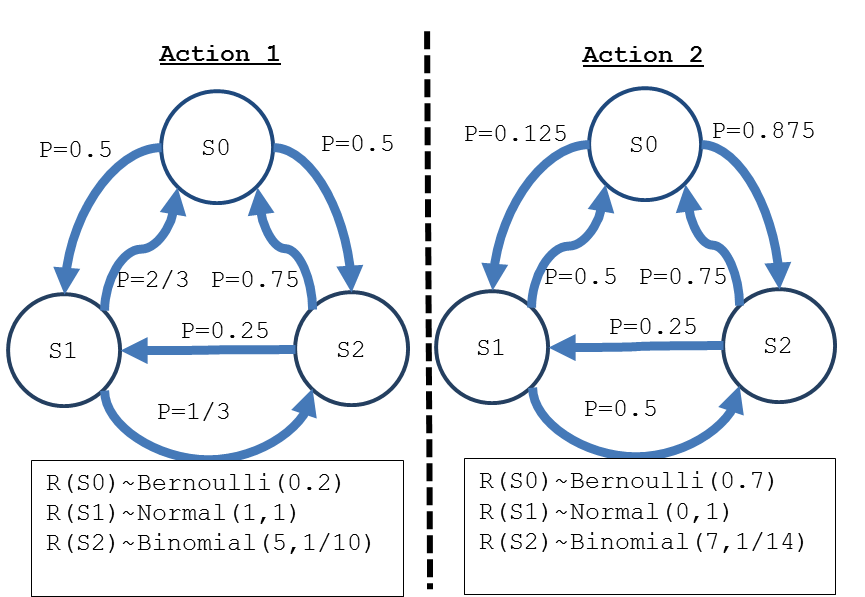
\includegraphics[width=0.8\textwidth]{hw3_a}
\end{center}
\begin{enumerate}
  \item You allow Jack to play a few rounds. Since 21 is his favorite number, Jack starts with the action 2, followed by the action 1 then again action 2 and so on. What is Jack's expected reward after 3 rounds (i.e., 3 actions)?
  \item Jack changes his strategy and starts a new game (at ${s_0}$) choosing the action to be either 1 or 2 with equal probability. What will be Jack's expected reward after 3 rounds now? What is the induced stationary policy over the states?
  \item Write and solve Bellman equations for 3 rounds. What is the optimal policy?
  \item Assuming each round there is a $\beta $ probability of getting thrown out of the casino, write down the infinite horizon cumulative reward. Conclude the connection between the discount factor and the death rate of a process.
  \item Write the Bellman equations for the infinite horizon discounted case in this problem.
\end{enumerate}
\end{exercise}

\begin{exercise}[\textbf{Modeling an Inventory MDP}]
In this question we will model resource allocation problems as MDPs. For each given scenario, write down what are the corresponding states, actions, state-transitions and reward. Also, write down a suitable performance criteria.

\textbf{Remark:} there may be multiple ways to model each scenario. Write down what you think is the most reasonable.

\begin{enumerate}
  \item Consider managing a hot-dog stand. At each hour, starting from 08:00, you decide how many hot-dogs to order from your supplier, each costing $c$, and they arrive instantly. At each hour, the number of hot-dog costumers is a random variable with Poisson distribution with rate $r$, and each customer buys a hot-dog for price $p$. At time 22:00 you close the stand, and throw away the remaining unsold hot-dogs.
  \item Consider scenario (1), but now each supplied hot-dog can only stay fresh for three hours, and then it has to be thrown away.
  \item Consider scenario (1), but now during 12:00-14:00 costumers arrive at double rate.
  \item Consider scenario (1), but now the stand is operated non-stop 24 hours a day. In addition, there is a yearly inflation ratio of 3\%.
  \item Consider scenario (4), but now during 12:00-14:00 costumers arrive at double rate.
\end{enumerate}
\end{exercise}

\begin{exercise}
Prove the following equality (from Section \ref{s:FP_VF} of the lecture notes)
\begin{align*}
V_{}^\pi (s) &\buildrel \Delta \over = {E^\pi }(\sum\limits_{t = 0}^\infty  {{\gamma ^t}r({s_t},{a_t})} |{s_0} = s)\\
 &= {E^\pi }(\sum\limits_{t = 1}^\infty  {{\gamma ^{t - 1}}r({s_t},{a_t})} |{s_1} = s).
\end{align*}
\end{exercise}

\begin{exercise}[\textbf{The $c \mu$ rule}]\label{ex:c_mu}
Assume $N$ jobs are scheduled to run on a single server. At each time step $(t=0,1,2,�)$, the sever may choose one of the remaining unfinished jobs to process. If job $i$ is chosen, then with probability ${\mu _i} > 0$ it will be completed, and removed from the system; otherwise the job stays in the system, and remains in an unfinished state.

Notice that the job service is memoryless - the probability of a job completion is independent of the number of times it has been chosen.
Each job is associated with a waiting cost ${c_i} > 0$ that is paid for each time step that the job is still in the system. The server's goal is minimizing the total cost until all jobs leave the system.
\begin{enumerate}
  \item Describe the problem as a Markov decision process. Write Bellman's equation for this problem.
  \item Show that the optimal policy is choosing at each time step ${i^*} = \argmax_i {c_i}{\mu _i}$ (from the jobs that are still in the system).

  \textbf{Hint: }Compute the value function for the proposed policy and show that it satisfies the Bellman equation.
\end{enumerate}
Remark: the $c\mu $ law is a fundamental result in queuing theory, and applies also to more general scenarios.
\end{exercise}

\begin{exercise}[\textbf{Blackjack}]
Black Jack is a popular casino card game. The object is to obtain a hand with the maximal sum of card values, but without exceeding 21. All face cards count as 10, and the ace counts as 11 (unlike the original game). In our version, each player competes independently against the dealer, and the card deck is infinite (i.e., the probability of drawing a new card from the deck does not depend on the cards in hand).

The game begins with two cards dealt to the player and one to the dealer. If the player starts with 21 it is called a natural (an ace and a 10 card), and he wins (reward = 1).
If the player did not start with 21 he can request additional cards one by one (hits), until he either chooses to stop (sticks) or exceeds 21 (goes bust). If he goes bust, he loses (reward=-1), if he sticks - then it becomes the dealer's turn.
The dealer first draws a second card. Then, the dealer hits or sticks according to a fixed policy: he sticks on any sum of 17 or greater.
If the dealer busts, then the player wins (reward = 1). Otherwise, the outcome--win, lose, or draw--is determined by whose final sum is closer to 21.

We represent a state as $\left( {X,Y} \right)$ where $X$  is the current player sum and $Y$ is the dealer's first card.
\begin{enumerate}
  \item Describe the problem as a Markov decision process. What is the size of the state space?
  \item Use value iteration to solve the MDP. Plot the optimal value function ${V^*}$ as a function of $\left( {X,Y} \right)$.
  \item Use the optimal value function to derive an optimal policy. Plot the optimal policy as follows: for each value of the dealer's card ($Y$), plot the minimal value for which the policy sticks.
\end{enumerate}
Here's an example of the plots you should provide (the values should be different though)
\begin{center}
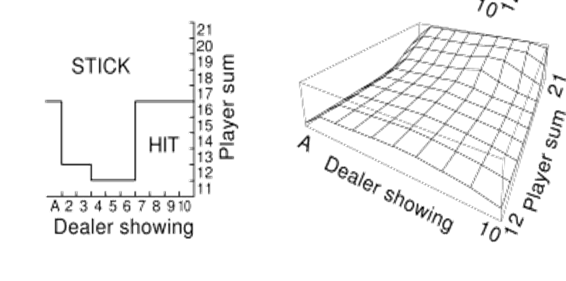
\includegraphics[width=0.7\textwidth]{hw3_b}
\end{center}
\end{exercise}

\begin{exercise}[\textbf{DP operator not contracting in Euclidean norm}]
Recall the fixed-policy DP operator ${T^\pi }$ defined as (see Section \ref{ss:DP_op})
\[\left( {{T^\pi }\left( J \right)} \right)\left( s \right) = r\left( {s,\pi (s)} \right) + \gamma {\sum _{s' \in S}}p\left( {s'|s,\pi (s)} \right)J\left( {s'} \right),\]
where $\gamma  < 1$. We have seen that ${T^\pi }$ is a contraction in the sup-norm. Show that ${T^\pi }$ is not necessarily a contraction in the Euclidean norm.

\textbf{Hint: }one possible approach is to consider the following 2-state MDP, and choose appropriate values for ${p_1},{p_2},\gamma $ to obtain a contradiction to the contraction property.
\begin{center}
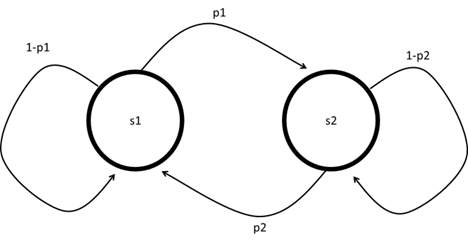
\includegraphics[width=0.6\textwidth]{hw3_c}
\end{center}
\end{exercise}

\begin{exercise}[\textbf{Contraction of ${\left( {{T^*}} \right)^k}$ }]
Recall that the Bellman operator ${T^*}$  defined by
\[\left( {{T^*}\left( J \right)} \right)\left( s \right) = {\max _{a \in A}}\left\{ {r\left( {s,a} \right) + \gamma {\sum _{s' \in S}}p\left( {s'|s,a} \right)J\left( {s'} \right)} \right\}\]
is a $\gamma$-contraction. We will show that ${\left( {{T^*}} \right)^k}$ is a ${\gamma ^k}$-contraction.
\begin{enumerate}
  \item For some $J$  and $\bar J$ let $c = {\max _s}\left| {J\left( s \right) - \bar J\left( s \right)} \right|$. Show that
\begin{equation}\label{eq:ex3a}
{\left( {{T^*}} \right)^k}\left( {J - ce} \right) \le {\left( {{T^*}} \right)^k}\left( {\bar J} \right) \le {\left( {{T^*}} \right)^k}\left( {J + ce} \right),
\end{equation}
where $e$ is a vector of ones.
  \item Now use \eqref{eq:ex3a} to show that  ${\left( {{T^*}} \right)^k}$ is a ${\gamma ^k}$-contraction.
\end{enumerate}
\end{exercise}

\begin{exercise}[\textbf{Second moment and variance of return}]
In the lectures we have defined the value function $V_{}^\pi (s)$ as the expected discounted return when starting from state $s$ and following policy $\pi $,
\[V_{}^\pi (s) = {E^{\pi ,s}}(\sum\limits_{t = 0}^\infty  {{\gamma ^t}r({s_t},{a_t})} ).\]
We have seen that $V_{}^\pi (s)$ satisfies a set of  $|S|$ linear equations (Bellman equation)
\[{V^\pi }{\kern 1pt} (s) = r(s,\pi (s)) + \gamma \sum\nolimits_{s' \in S} {p(s'|s,\pi (s)){V^\pi }(s')} \;,\quad \;s \in S.\]
We now define $M_{}^\pi (s)$ as the second moment of the discounted return when starting from state $s$ and following policy $\pi $,
\[M_{}^\pi (s) = {E^{\pi ,s}}\left( {{{\left( {\sum\limits_{t = 0}^\infty  {{\gamma ^t}r({s_t},{a_t})} } \right)}^2}} \right).\]
\begin{enumerate}
  \item We will show that $M_{}^\pi (s)$ satisfies a 'Bellman like' set of equations. Write an expression for $M_{}^\pi (s)$ that has a linear dependence on $M_{}^\pi $ and  $V_{}^\pi $.

\textbf{Hint:} start by following the derivation of the Bellman equation for $V_{}^\pi .$
  \item How many equations are needed to solve in order to calculate $M_{}^\pi (s)$ for all $s \in S$ ?
  \item We now define $W_{}^\pi (s)$ as the variance of the discounted return when starting from state $s$ and following policy $\pi $,
\[W_{}^\pi (s) = {\rm{Va}}{{\rm{r}}^{\pi ,s}}\left( {\sum\limits_{t = 0}^\infty  {{\gamma ^t}r({s_t},{a_t})} } \right).\]
Explain how $W_{}^\pi (s)$ may be calculated.
\end{enumerate}
\end{exercise}

\begin{exercise}
Consider the modified policy iteration scheme of Section \ref{ss:mod_PI}.
Show that extreme values of ${m_k}$ (which?) reduce this algorithm to the standard Value Iteration or Policy Iteration.
\end{exercise}
